\documentclass[UTF8,aspectratio=169,10pt]{ctexbeamer}

\usetheme{Madrid}
\usecolortheme{dolphin}
\setbeamertemplate{navigation symbols}{}
\setbeamertemplate{footline}[frame number]

\usepackage{booktabs}
\usepackage{tabularx}
\usepackage{array}
\usepackage{adjustbox}
\usepackage{graphicx}
\usepackage{xcolor}

\graphicspath{{assets/}}

\definecolor{pgsaBlue}{RGB}{32,74,135}
\definecolor{pgsaGreen}{RGB}{44,129,88}
\definecolor{pgsaOrange}{RGB}{190,104,33}
\definecolor{pgsaGray}{RGB}{82,90,99}

\newcommand{\keyword}[1]{\textcolor{pgsaBlue}{\textbf{#1}}}
\newcommand{\metric}[1]{\textcolor{pgsaGreen}{\textbf{#1}}}
\newcommand{\warn}[1]{\textcolor{pgsaOrange}{\textbf{#1}}}
\newcommand{\smallsource}[1]{\vspace{0.4em}{\scriptsize\textcolor{pgsaGray}{Source: #1}}}
\newcommand{\fitfig}[2]{\includegraphics[width=#1\textwidth,height=0.70\textheight,keepaspectratio]{#2}}

% Speaker notes are hidden in the normal slide PDF.
% To render a notes version, enable a Beamer notes option in the compile environment,
% for example: \setbeameroption{show notes on second screen=right}
\setbeameroption{hide notes}

\title[二阶段组装效率与硬件适配]{并行整体刚度矩阵组装：二阶段组装效率与硬件适配评估}
\subtitle{面向 mentor 下一步意见的实验整理}
\author{Jiang Haohua}
\date{2026-05-14}

\begin{document}

\begin{frame}
  \titlepage
\end{frame}
\note{
开场时先说明这不是重新介绍整个项目，而是针对 mentor 最近给出的两个方向做一次阶段性整理。标题里的“二阶段组装”指符号组装和数值组装分开；“硬件适配”指线程数、物理核、P/E core profile 和 OpenMP 绑定设置这些因素。这里要先给出平台定位：Intel Core Ultra 7 265KF 是这份材料的主要 CPU 平台，因为 x86/Intel 用户基数最大；Apple M4 Max 是本机复现、符号/无符号串行评估和跨平台对照平台。
}

\begin{frame}{这次先把效率问题和 Intel 平台优先级分清楚}
\begin{columns}[T,onlytextwidth]
\begin{column}{0.50\textwidth}
\textbf{效率问题}
\begin{itemize}
  \item 单次组装和多次组装要分开看。
  \item 有符号组装和无符号直接组装要分开比。
  \item 重点不是换一个名字，而是看稀疏结构能不能复用。
\end{itemize}
\end{column}
\begin{column}{0.46\textwidth}
\textbf{硬件问题}
\begin{itemize}
  \item Intel 是优先展示平台，Apple 是复现和对照平台。
  \item 线程数增加不等于一定加速。
  \item Intel 的 P/E-core 用 \texttt{taskset} 做实际 affinity restriction。
  \item Apple 的 QoS profile 只能作为调度偏置实验。
\end{itemize}
\end{column}
\end{columns}
\end{frame}
\note{
这一页的目的，是把 mentor 的四个问题收敛成两条主线，同时先把平台优先级说清楚。左边讲效率：单次和多次组装为什么不同，因为符号阶段如果能复用，多次组装时预处理成本会被摊薄。右边讲硬件：Intel 是后续面向主要用户群体的优先平台，所以硬件适配部分要先讲 Intel Core Ultra 7 265KF 的 full-host、P-core-only 和 E-core-only 实测结果。Apple M4 Max 仍然重要，但它承担的是本机复现和跨平台边界说明，不应该盖过 Intel 主线。
}

\begin{frame}{实验平台先固定，后面每个数字才可比较}
\begin{columns}[T,onlytextwidth]
\begin{column}{0.53\textwidth}
\textbf{共享数据结构}
\begin{itemize}
  \item \texttt{Mesh}: 节点、单元和 DOF 映射。
  \item \texttt{CsrMatrix}: 全局刚度矩阵的稀疏结构和值。
  \item \texttt{AssemblyPlan}: 每个单元的 DOF 和写入位置。
  \item \texttt{relative\_l2 <= 1e-8}: 数值正确性检查。
\end{itemize}
\end{column}
\begin{column}{0.43\textwidth}
\textbf{参与比较的 CPU 算法}
\begin{itemize}
  \item \texttt{cpu\_serial}
  \item \texttt{cpu\_atomic}
  \item \texttt{cpu\_private\_csr}
  \item \texttt{cpu\_coo\_sort\_reduce}
  \item \texttt{cpu\_graph\_coloring}
  \item \texttt{cpu\_row\_owner}
\end{itemize}
\end{column}
\end{columns}
\smallsource{README.md; docs/cpu; benchmark and symbolic evaluation source files}
\end{frame}
\note{
这一页解释“为什么这些实验可以放在一起讲”。左边是平台层：所有算法都在同一个 Mesh、同一个 CSR 矩阵和同一个 AssemblyPlan 上比较，所以差别主要来自组装策略和并行策略，而不是输入格式不同。AssemblyPlan 里存了两个关键东西：单元的全局 DOF 列表，以及局部刚度矩阵每个条目该写到 CSR values 的哪个位置。\texttt{relative\_l2} 是正确性指标，表示候选矩阵和 serial baseline 的相对二范数误差；阈值 1e-8 用来排除“跑得快但结果错”的情况。右边列出算法，讲的时候不用逐个展开，只要说明后面图里会出现这些名字。
}

\begin{frame}{符号阶段和数值阶段各做一半工作}
\begin{columns}[T,onlytextwidth]
\begin{column}{0.48\textwidth}
\textbf{符号阶段}
\begin{itemize}
  \item 全局矩阵的 CSR sparsity pattern。
  \item 每个单元的全局 DOF 列表。
  \item 每个 \texttt{Ke(i,j)} 对应的 CSR value index。
\end{itemize}
\end{column}
\begin{column}{0.48\textwidth}
\textbf{数值阶段}
\begin{itemize}
  \item 读取坐标和材料参数。
  \item 对 Tet4 计算体积、形函数梯度和 $B^TDB$。
  \item 按 scatter 位置把 \texttt{Ke} 累加到全局矩阵。
\end{itemize}
\end{column}
\end{columns}
\begin{alertblock}{这里的边界}
网格拓扑和 DOF 编号不变时，符号结果可以保留；材料状态或迭代状态变化时，只重复数值阶段。
\end{alertblock}
\end{frame}
\note{
这一页把符号阶段和数值阶段放在一起讲。CSR 是 compressed sparse row，全局刚度矩阵很稀疏，不适合存成完整 dense matrix。符号阶段先确定哪些位置会非零，并把行偏移、列索引这些结构建好。scatter 指的是局部矩阵条目 Ke(i,j) 写回全局 CSR values 数组的位置。数值阶段才计算 Ke，也就是 element stiffness matrix。\texttt{physics\_tet4} 里，Tet4 的局部刚度来自体积、应变位移矩阵 B、材料矩阵 D，最后形成 $B^T D B$，再乘以体积。$B^TDB$ 可以讲成：把材料本构和形函数梯度合起来，得到单元内部自由度之间的刚度关系。为什么可以重复数值阶段？因为很多有限元问题里，网格和 DOF 编号不变，只是材料状态、载荷步或迭代状态变化。
}

\begin{frame}{mentor 示例和当前 C++ 实现可以逐项对上}
\begin{adjustbox}{max width=\textwidth}
\begin{tabular}{lll}
\toprule
Mentor 示例概念 & 当前 C++ 实现 & 在项目里的作用 \\
\midrule
\texttt{build\_symbolic\_pattern} & \texttt{CsrMatrix::build\_sparsity} & 生成 CSR pattern \\
\texttt{cellDofsCache} & \texttt{AssemblyPlan::dofs} & 缓存每个单元的全局 DOF \\
\texttt{allocate\_global\_matrix} & \texttt{CsrMatrix} 清零并复用 values & 结构不变，只更新数值 \\
\texttt{assemble\_numeric} & \texttt{cpu\_serial} 等 assembler & 计算 \texttt{Ke} 并写回全局矩阵 \\
无直接对应项 & \texttt{AssemblyPlan::scatter} & 提前保存 CSR 写入位置 \\
section / closure & 固定每节点 3 DOF & 当前先不引入高阶 DOF 抽象 \\
\bottomrule
\end{tabular}
\end{adjustbox}
\smallsource{docs/cpu/symbolic\_numeric\_assembly.md; results/2026-05-11-symbolic-numeric/symbolic\_numeric\_eval\_report.md}
\end{frame}
\note{
这一页说明我们没有机械照搬 mentor 的 MATLAB 示例，而是把示例里的思想映射到现有 C++ 平台。第一行是稀疏结构，第二行是单元 DOF 缓存，第三行是全局矩阵预分配，第四行是数值组装。第五行很关键：C++ 里多了 AssemblyPlan::scatter，这比教学示例更接近高性能实现，因为它把局部条目到 CSR 位置的映射也缓存下来。最后一行说明 section/closure 这类 PETSc 风格抽象暂时没有引入，因为当前单元是固定每节点 3 个位移自由度，还没有做高阶单元或边自由度。
}

\begin{frame}{效率表和硬件图来自两类平台数据}
\begin{columns}[T,onlytextwidth]
\begin{column}{0.40\textwidth}
\textbf{固定算例}
\begin{itemize}
  \item nodes = \metric{228384}
  \item elements = \metric{1113684}
  \item dofs = \metric{685152}
  \item element = \texttt{Tet4}
  \item kernel = \texttt{physics\_tet4}
\end{itemize}
\end{column}
\begin{column}{0.56\textwidth}
\textbf{平台边界}
\begin{itemize}
  \item 符号/无符号效率表：Apple M4 Max，macOS arm64，Clang 21.0.0，OpenMP 202011，physical/logical = 14/14。
  \item 硬件适配主平台：Intel(R) Core(TM) Ultra 7 265KF，Linux x86\_64，GCC 13.3，OpenMP 201511，physical/logical = 20/20。
  \item Apple 时间不替代 Intel 绝对性能；Intel 图用于回答主要用户平台上的线程和核心 profile 问题。
\end{itemize}
\end{column}
\end{columns}
\begin{block}{这样做的原因}
固定网格、单元类型和核函数后，先比较符号结构复用的算法收益；再用 Intel 实测图解释主要 CPU 平台上的硬件适配边界。
\end{block}
\end{frame}
\note{
这一页要解释实验设置和数据边界。WindTurbineHub 是真实工程网格，规模足够大，能体现稀疏结构构建和全局写入的成本。nodes 是节点数，elements 是单元数，dofs 是自由度数；这里每个节点 3 个位移自由度，所以 DOF 数约等于节点数乘以 3。kernel 选 \texttt{physics\_tet4}，是因为这组比较要回答真实 Tet4 物理组装成本，而不是只看 synthetic assembly overhead。右边要讲清楚：符号/无符号效率表来自 Apple M4 Max，本质回答的是“复用稀疏结构是否有价值”；Intel Core Ultra 7 265KF 是硬件适配的主要平台，后面用它的 full-host、P-core-only 和 E-core-only 结果回答线程数和核心 profile 问题。不能把 Apple 的组装时间写成 Intel 的绝对性能。
}

\begin{frame}{单次组装也受益，多次组装收益更明显}
\begin{adjustbox}{max width=\textwidth}
\begin{tabular}{rrrrrrrr}
\toprule
组装次数 & 符号总耗时 & 数值/次 & 符号复用摊销总耗时 & 直接生成/次 & 直接排序归并/次 & 无符号直接总耗时 & 收益 \\
 & ms & ms & ms & ms & ms & ms & \\
\midrule
1  & 3200.968 & 617.818 & 3818.786 & 770.372 & 5505.827 & 6276.199 & \metric{1.644x} \\
3  & 3195.067 & 568.143 & 1633.165 & 593.735 & 5228.634 & 5822.369 & \metric{3.565x} \\
10 & 3256.337 & 575.691 & 901.325  & 549.004 & 5147.784 & 5696.788 & \metric{6.320x} \\
30 & 3252.907 & 578.315 & 686.745  & 516.919 & 5035.935 & 5552.854 & \metric{8.086x} \\
\bottomrule
\end{tabular}
\end{adjustbox}

\vspace{0.5em}
符号复用的优势来自两部分：少做结构分析，少做直接贡献的全局排序归并。
\smallsource{results/2026-05-11-symbolic-numeric/symbolic\_numeric\_eval\_report.md; Apple M4 Max/macOS arm64 source run}
\end{frame}
\note{
这页是核心结果，讲慢一点。第一列是同一个符号结构下做几次数值组装。符号总耗时包括 CSR 构建和 scatter plan 构建。数值/次是每次 \texttt{physics\_tet4} 组装的平均时间。符号复用摊销总耗时是把一次符号成本加上多次数值成本后除以组装次数。右边三列是无符号直接组装：先生成所有 row、col、value 贡献，再排序归并。最后一列收益是无符号直接总耗时除以符号复用摊销总耗时。要强调两个数字：一次组装已经有 1.644x，说明即使只组装一次，排序归并也很贵；30 次达到 8.086x，说明多次迭代场景下符号复用特别有价值。同时要补一句边界：这组收益数字来自 Apple M4 Max，它回答的是“复用稀疏结构是否有价值”，不是 Intel 绝对性能排名。
}

\begin{frame}{单次和多次组装对应两种使用场景}
\begin{columns}[T,onlytextwidth]
\begin{column}{0.48\textwidth}
\textbf{单次组装}
\begin{itemize}
  \item 符号复用路径：\metric{3818.786 ms}
  \item 无符号直接路径：\metric{6276.199 ms}
  \item 主要差距来自直接路径的排序归并。
\end{itemize}
\end{column}
\begin{column}{0.48\textwidth}
\textbf{多次组装}
\begin{itemize}
  \item 3 次：\metric{3.565x}
  \item 10 次：\metric{6.320x}
  \item 30 次：\metric{8.086x}
  \item 更贴近 Newton iteration 或 time stepping。
\end{itemize}
\end{column}
\end{columns}
\begin{alertblock}{对项目有用的结论}
如果网格和 DOF 编号不变，组装流程应该尽量保留符号结构，把后续工作压到数值阶段。
\end{alertblock}
\end{frame}
\note{
这一页把上一张表翻译成实际使用场景。单次组装对应最保守的情况，也就是只组装一次全局刚度矩阵。这里符号复用仍然快，因为直接生成贡献后排序归并的成本太高。多次组装对应非线性求解、参数扫描或时间步进，稀疏结构不变，只是数值变，这时符号成本被摊销，所以收益越来越大。讲这页时可以说：mentor 问单次和多次组装，我的结论是两者都值得做符号结构，但多次组装更能体现二阶段路线的优势。
}

\begin{frame}{有符号和无符号的区别在写入路径}
\begin{columns}[T,onlytextwidth]
\begin{column}{0.50\textwidth}
\textbf{有符号组装}
\begin{itemize}
  \item CSR pattern 先固定。
  \item 单元 DOF 先缓存。
  \item \texttt{Ke(i,j)} 写到哪里先算好。
  \item 数值阶段直接按位置累加。
\end{itemize}
\end{column}
\begin{column}{0.46\textwidth}
\textbf{无符号直接组装}
\begin{itemize}
  \item 每次生成所有 \texttt{(row,col,value)}。
  \item 每次对贡献做排序和 reduce。
  \item WindHub 单次排序归并约 \metric{5.5 s}。
  \item transient memory 约 \metric{2.39 GiB}。
\end{itemize}
\end{column}
\end{columns}
\begin{block}{比较的实质}
这里比较的是“是否提前知道全局稀疏写入位置”，不是比较两个函数名。
\end{block}
\end{frame}
\note{
这一页回答有符号和无符号的本质差别。左边有符号路径，先知道全局矩阵有哪些非零项，也知道局部 Ke 的每个条目要累加到哪个 CSR values 下标。右边无符号路径，每次都把所有单元贡献摊开成三元组，然后排序，把相同 row 和 col 的贡献加起来。WindHub 这个算例里，直接路径的排序归并单次大约 5.5 秒，这是表里 direct sort-reduce 的数量级。transient memory 是中间三元组占用的临时内存，约 2.39 GiB。这里要让 mentor 看到：符号阶段不仅是理论概念，也直接减少了运行时的数据搬运和排序工作。
}

\begin{frame}{控制实验说明：重建符号结构不是推荐做法}
\begin{adjustbox}{max width=\textwidth}
\begin{tabular}{rrrrrrrr}
\toprule
组装次数 & 符号构建次数 & CSR 构建 & scatter plan & 符号总耗时 & 数值/次 & 摊销总耗时 & 相对无符号收益 \\
 & & ms & ms & ms & ms & ms & \\
\midrule
1  & 1  & 1714.238 & 1505.008 & 3219.246 & 594.023 & 3813.269 & 1.646x \\
3  & 3  & 1711.323 & 1435.719 & 3147.042 & 588.176 & 3735.218 & 1.559x \\
10 & 10 & 1661.970 & 1483.861 & 3145.832 & 598.086 & 3743.918 & 1.522x \\
30 & 30 & 1575.358 & 1306.344 & 2881.703 & 512.877 & 3394.580 & 1.636x \\
\bottomrule
\end{tabular}
\end{adjustbox}

\vspace{0.5em}
\texttt{symbolic\_rebuild\_serial} 用来排除一个误解：二阶段组装的价值不在“每次都拆成两步”，而在“符号结果可以复用”。
\end{frame}
\note{
这一页解释控制实验。\texttt{symbolic\_rebuild\_serial} 的做法是每次都重新构建 CSR pattern 和 scatter plan，然后只做一次数值组装。这个做法不是推荐方案，因为它没有复用符号结构。为什么还要做？因为它能说明二阶段路线的收益主要来自符号结果复用，而不是单纯把流程叫做 symbolic 和 numeric。表里可以看到，即便每次重建符号结构，它相对无符号直接路径仍有 1.5 到 1.6 倍左右收益，说明 CSR/scatter 路线本身比直接贡献排序归并更合理；但它远不如一次构建、多次复用的路线。
}

\begin{frame}{\texttt{simplified} 和 \texttt{physics\_tet4} 解决不同问题}
\begin{columns}[T,onlytextwidth]
\begin{column}{0.48\textwidth}
\textbf{Mesh topology}
\begin{itemize}
  \item \texttt{tet4} / Abaqus \texttt{C3D4}
  \item \texttt{hex8} / Abaqus \texttt{C3D8}
  \item 决定单元节点数与 DOF mapping。
\end{itemize}
\end{column}
\begin{column}{0.48\textwidth}
\textbf{Kernel mode}
\begin{itemize}
  \item \texttt{simplified}: synthetic local matrix。
  \item \texttt{physics\_tet4}: Tet4 物理刚度。
  \item 非 Tet4 使用 \texttt{physics\_tet4} 时会回退。
\end{itemize}
\end{column}
\end{columns}
\begin{alertblock}{讲结果时的边界}
\texttt{simplified} 看 assembly overhead；\texttt{physics\_tet4} 看更接近工程 Tet4/C3D4 的组装成本。两类图不要互相替代。
\end{alertblock}
\end{frame}
\note{
这一页处理一个容易混淆的问题：mesh topology 和 kernel mode 是两条轴。mesh topology 是 tet4 或 hex8，决定一个单元有几个节点和多少 DOF。kernel mode 是局部刚度矩阵怎么来。\texttt{simplified} 不看真实几何，只生成确定性的局部矩阵，它适合隔离全局 assembly 的写冲突、CSR scatter 和并行策略成本。\texttt{physics\_tet4} 会用 Tet4 的真实几何和 $B^TDB$ 算局部刚度，更适合工程解释。注意：如果输入是 Hex8 但要求 \texttt{physics\_tet4}，代码会回退到 \texttt{simplified}，所以不能把 \texttt{physics\_tet4} 当成任何网格都真实物理的开关。
}

\begin{frame}{真实 Tet4 物理组装下，最快点出现在 row-owner 路线}
\centering
\fitfig{0.94}{assets/windhub_physics_efficiency.png}
\smallsource{2026-04-28 repeat=3, threads=1..14, presentation\_charts\_12\_v2}
\end{frame}
\note{
这页展示 WindTurbineHub + \texttt{physics\_tet4} 的效率图。图里的每组柱或曲线比较不同算法在线程数变化下的组装时间、加速比和效率。\texttt{physics\_tet4} 意味着每个单元要做真实 Tet4 局部刚度计算，所以这个图更接近工程算例。讲图时重点看 best speedup 和对应线程数：\texttt{row\_owner} 在这组实验里达到最高加速比，约 5.35x，最快平均组装时间约 106.5 ms。\texttt{private\_csr} 也表现较好，但内存随线程数增加。\texttt{coo\_sort\_reduce} 在这个规模下明显不适合直接作为主力组装方法。
}

\begin{frame}{\texttt{simplified} 用来单独看全局组装开销}
\centering
\fitfig{0.94}{assets/windhub_simplified_efficiency.png}
\smallsource{2026-04-28 repeat=3, threads=1..14, presentation\_charts\_12\_v2}
\end{frame}
\note{
这页是 simplified kernel 的对照。\texttt{simplified} 不计算真实 Tet4 的 $B^TDB$，所以局部计算成本更低，图中更能突出全局稀疏写入、冲突处理、同步和内存流量这些 assembly overhead。讲这页时不要说它代表真实工程耗时，而要说它帮助我们看清楚“组装策略本身”的趋势。比如 \texttt{row\_owner} 和 \texttt{private\_csr} 的差异，不只是局部物理计算，而是写入策略、重复计算和内存归并之间的取舍。
}

\begin{frame}{正确性和内存要和速度一起看}
\begin{columns}[T,onlytextwidth]
\begin{column}{0.49\textwidth}
\centering
  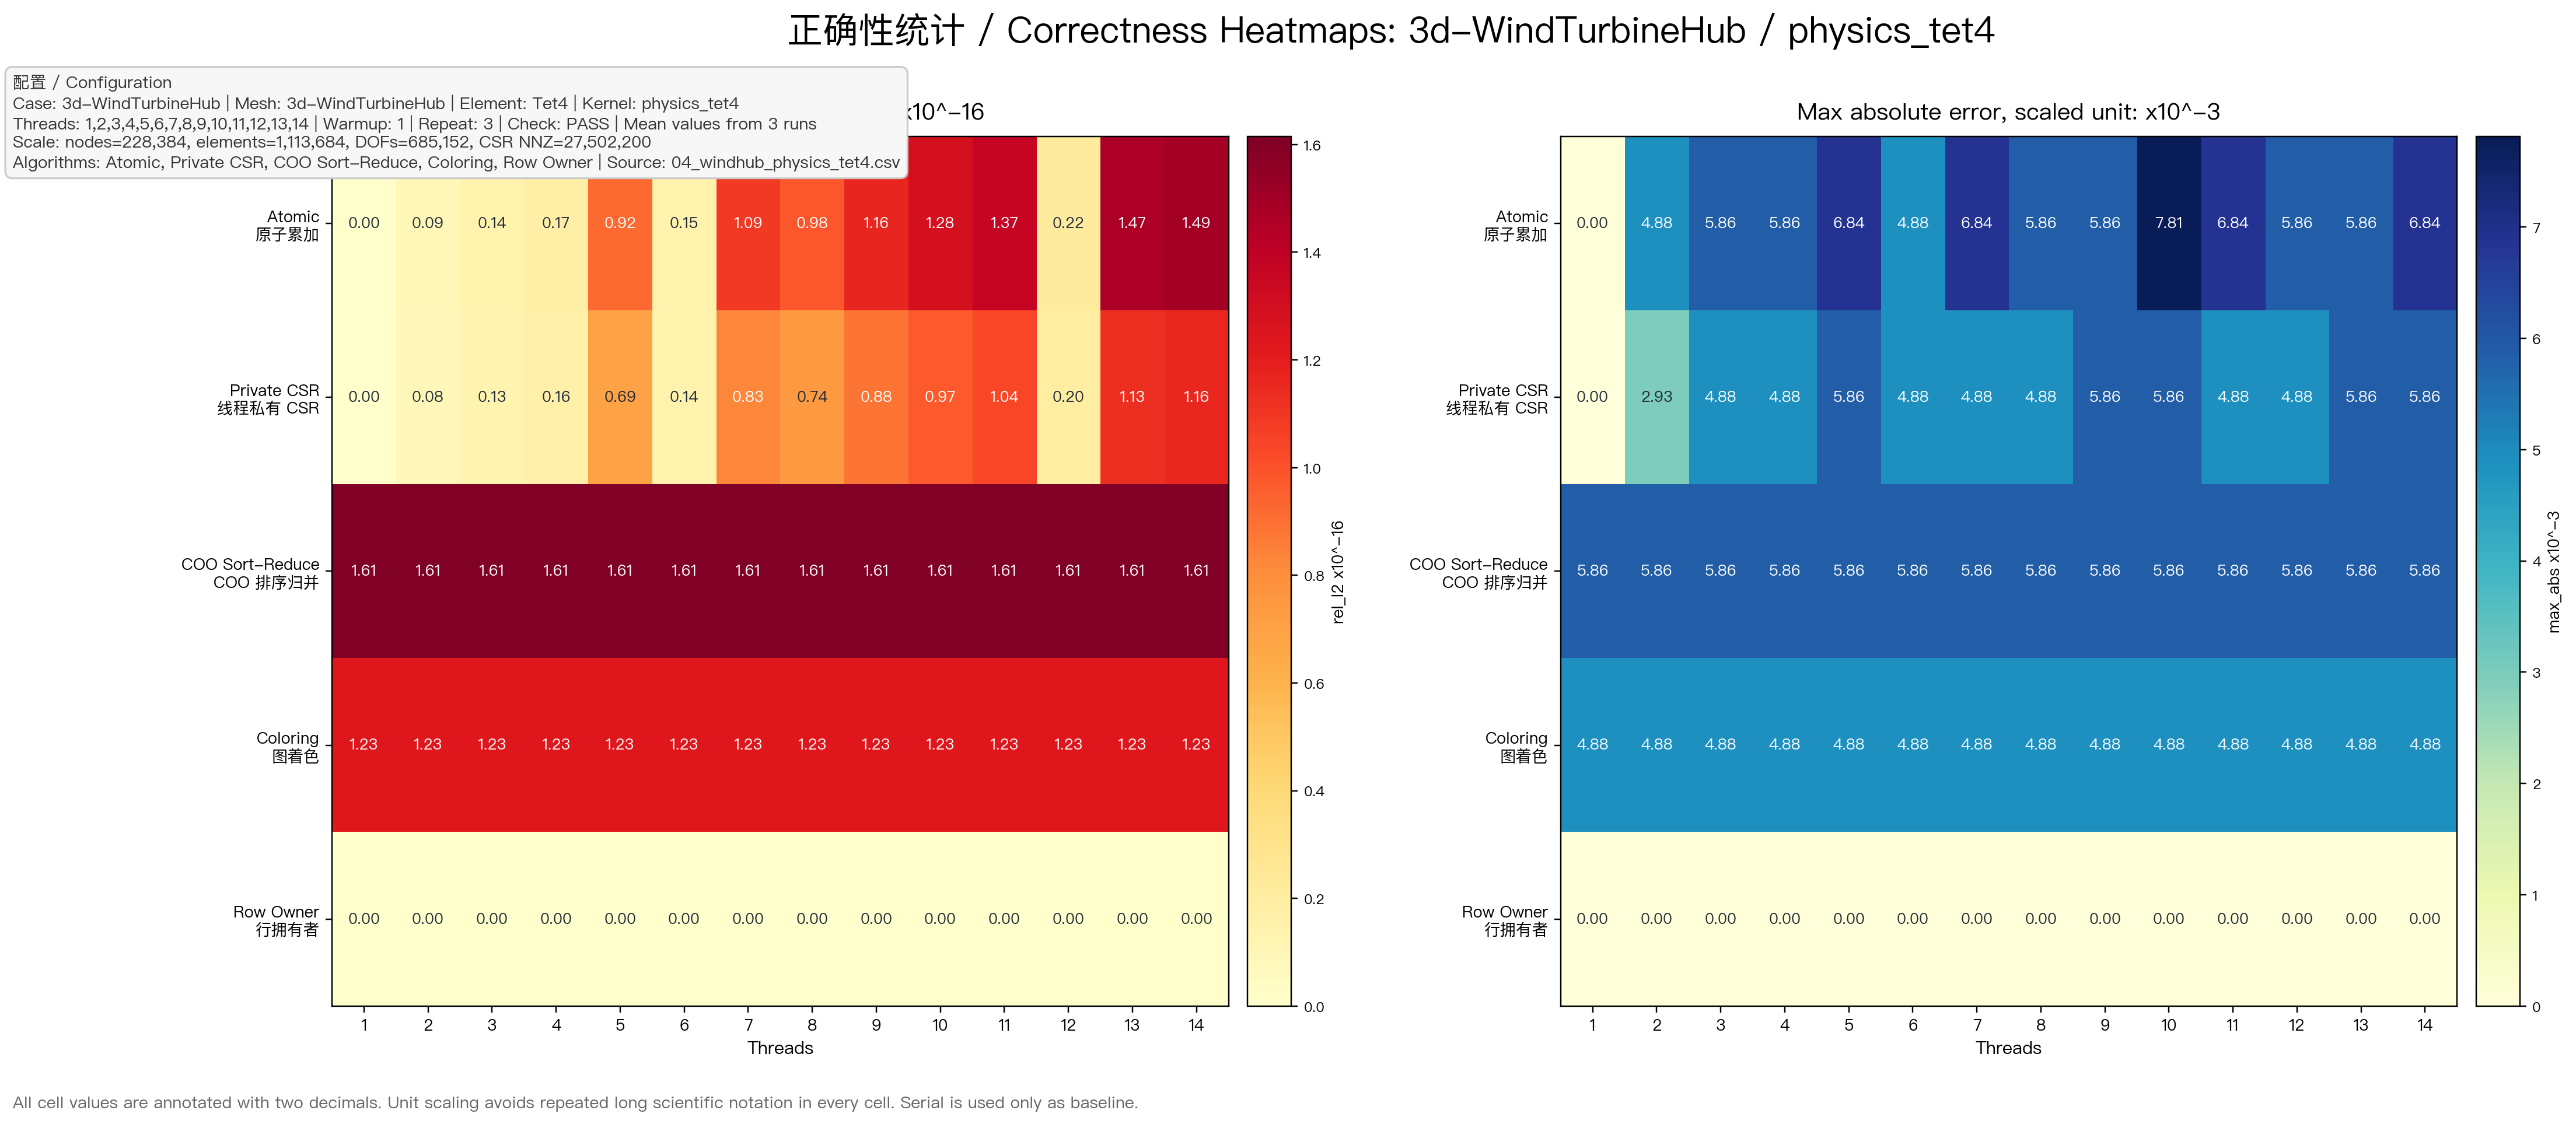
\includegraphics[width=\textwidth,height=0.68\textheight,keepaspectratio]{assets/windhub_physics_correctness.png}
\end{column}
\begin{column}{0.49\textwidth}
\centering
  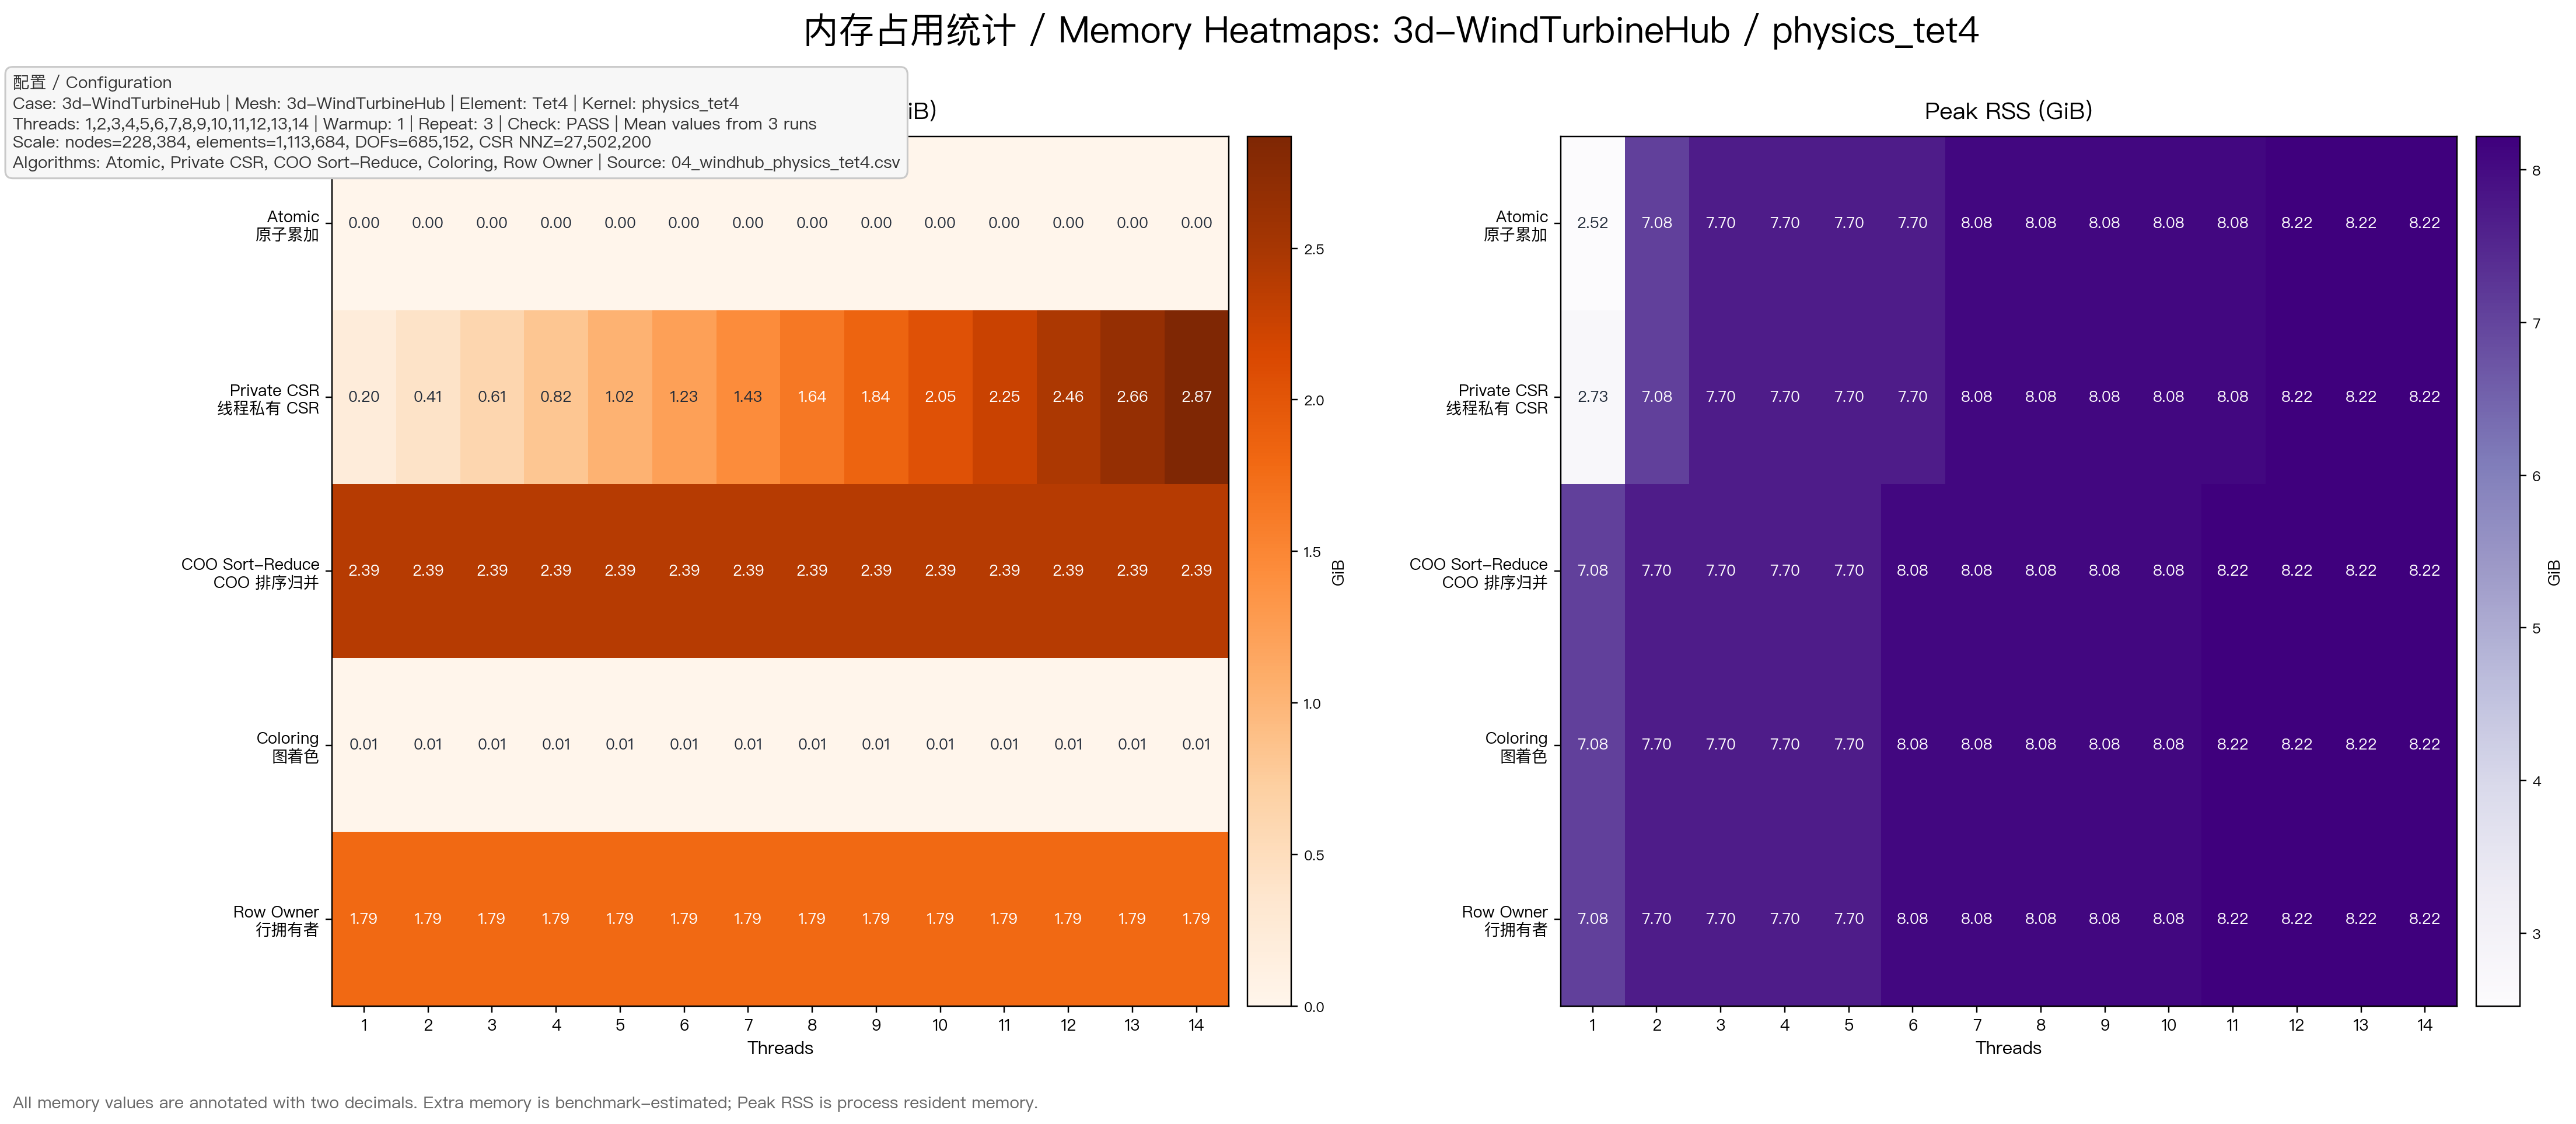
\includegraphics[width=\textwidth,height=0.68\textheight,keepaspectratio]{assets/windhub_physics_memory.png}
\end{column}
\end{columns}
\smallsource{WindTurbineHub physics\_tet4 correctness and memory heatmaps}
\end{frame}
\note{
这一页左边是正确性 heatmap，右边是内存 heatmap。正确性图主要看 \texttt{relative\_l2} 和 \texttt{max\_abs} 的量级，确认并行算法没有改变数学结果。\texttt{relative\_l2} 是相对二范数误差，越接近 0 越好；\texttt{max\_abs} 是单个矩阵条目的最大绝对差。右边内存图说明速度不是唯一指标。\texttt{private\_csr} 每个线程有自己的 CSR values 副本，所以额外内存随线程增加；\texttt{row\_owner} 避免 atomic，但可能有任务列表和重复计算带来的内存/计算代价。讲这页时要说明：选择算法时不能只看最快点，还要看内存和正确性边界。
}

\begin{frame}{硬件适配先从 Intel 主平台讲起}
\begin{columns}[T,onlytextwidth]
\begin{column}{0.50\textwidth}
\textbf{Intel Core Ultra 7 265KF}
\begin{itemize}
  \item Linux x86\_64, GCC 13.3, OpenMP 201511。
  \item physical/logical = 20/20。
  \item \texttt{full\_host}: 全 CPU 资源。
  \item \texttt{performance\_core\_only}: \texttt{taskset} restricted CPUs 0-7。
  \item \texttt{efficiency\_core\_only}: \texttt{taskset} restricted CPUs 8-19。
\end{itemize}
\end{column}
\begin{column}{0.46\textwidth}
\textbf{Apple M4 Max 对照}
\begin{itemize}
  \item macOS arm64, Clang 21.0.0, OpenMP 202011。
  \item physical/logical = 14/14。
  \item performance / efficiency 是 QoS-biased profile。
  \item Apple 没有和 Linux \texttt{taskset} 等价的公开硬绑核接口。
\end{itemize}
\end{column}
\end{columns}
\end{frame}
\note{
这一页进入硬件适配。先讲 Intel，因为这是面向主要用户群体的优先平台。Intel 这组结果来自 Linux x86\_64、GCC 13.3、OpenMP 201511，CPU 是 Intel Core Ultra 7 265KF，记录里 physical/logical = 20/20。这里的三个 profile 是同一个 CPU 上的资源限制：\texttt{full\_host} 用全 CPU；\texttt{performance\_core\_only} 通过 \texttt{taskset} restricted CPUs 0-7；\texttt{efficiency\_core\_only} 通过 \texttt{taskset} restricted CPUs 8-19。右边 Apple 只作为对照：它的 QoS-biased profile 说明调度偏置敏感性，但不是硬绑核。口头上要明确：Intel 和 Apple 的平台机制不同，不能把两个 profile 名字当成同一种硬件实验。
}

\begin{frame}{Intel: \texttt{taskset} 下的 P/E-core 资源限制}
\centering
\fitfig{0.93}{assets/core_profile_intel_u7_265kf.png}
\smallsource{cross-platform-v1/figures; Linux taskset affinity-restricted P/E-core profiles}
\end{frame}
\note{
这页讲 Intel Core Ultra 7 265KF 的 core-profile 图。图里比较 \texttt{full\_host}、\texttt{performance\_core\_only} 和 \texttt{efficiency\_core\_only} 三种资源 profile。\texttt{full\_host} 可以使用整个 CPU；P-core-only 通过 taskset 限制在 CPU 0-7；E-core-only 限制在 CPU 8-19。讲图时强调：这不是在说某个算法天生只适合 P-core 或 E-core，而是在说可用核心集合变化后，最好线程数和最优时间会变化。对于 \texttt{private\_csr} 这种内存压力大的算法，核心类型和内存带宽都会影响结果；对于 atomic 和 \texttt{row\_owner}，也会受写冲突和负载均衡影响。
}

\begin{frame}{Intel P-core-only: \texttt{taskset} restricted CPUs 0-7}
\centering
\fitfig{0.93}{assets/intel_pcore_bound_dashboard.png}
\smallsource{2026-05-12-thread-scaling-linux-intel-pcore}
\end{frame}
\note{
这页把 Intel P-core-only 从附录提升到硬件主线里讲。它使用 \texttt{taskset -c 0-7}，把进程限制在 Intel Core Ultra 7 265KF 的 P-core CPU id 范围内；图里展示 bound 环境下各算法随线程数变化的时间、加速比、效率和内存。讲的时候重点不是“P-core 一定最好”，而是说明当可用核心集合被限制到高性能核心时，最优线程数、效率曲线和内存压力会一起变化。这里和 Intel \texttt{full\_host}、Intel E-core-only 做同平台对照，不和 Apple QoS 图做绝对速度排名。
}

\begin{frame}{Intel E-core-only: \texttt{taskset} restricted CPUs 8-19}
\centering
\fitfig{0.93}{assets/intel_ecore_bound_dashboard.png}
\smallsource{2026-05-12-thread-scaling-linux-intel-ecore}
\end{frame}
\note{
这页是 Intel E-core-only 主线结果。它使用 \texttt{taskset -c 8-19}，把进程限制在 Intel Core Ultra 7 265KF 的 E-core CPU id 范围内。这个图的用途是解释：核心数量更多不一定自动带来更短组装时间，因为单核能力、内存系统、写冲突和算法负载均衡都会影响最终结果。如果 mentor 问 P-core 和 E-core 差异，可以把这页和上一页连在一起讲：Intel 平台已经有实际 affinity restriction 结果，Apple QoS 图只是补充说明跨平台调度边界。
}

\begin{frame}{Apple: QoS 只能说明调度偏置，不能当硬绑核}
\centering
\fitfig{0.93}{assets/core_profile_apple_m4_max.png}
\smallsource{cross-platform-v1/figures; macOS QoS-biased sensitivity profiles, not hard-pinned affinity}
\end{frame}
\note{
这页讲 Apple M4 Max。Apple 有 10 个性能核心和 4 个能效核心，但 macOS 不提供和 Linux taskset 等价的公开硬绑核方式。这里的 performance profile 是正常前台调度并把线程范围限制在性能核心数量附近；efficiency profile 使用 taskpolicy background 做 QoS 偏置，并把线程范围限制在能效核心数量附近。讲图时一定说明：这张图可以说明调度策略和核心资源偏置对结果很敏感，但不能把它解释为严格 P-core-only 和 E-core-only 的硬件吞吐比较。
}

\begin{frame}{超过物理核后的线程数是过量订阅，不是 SMT 收益}
\begin{columns}[T,onlytextwidth]
\begin{column}{0.49\textwidth}
\centering
  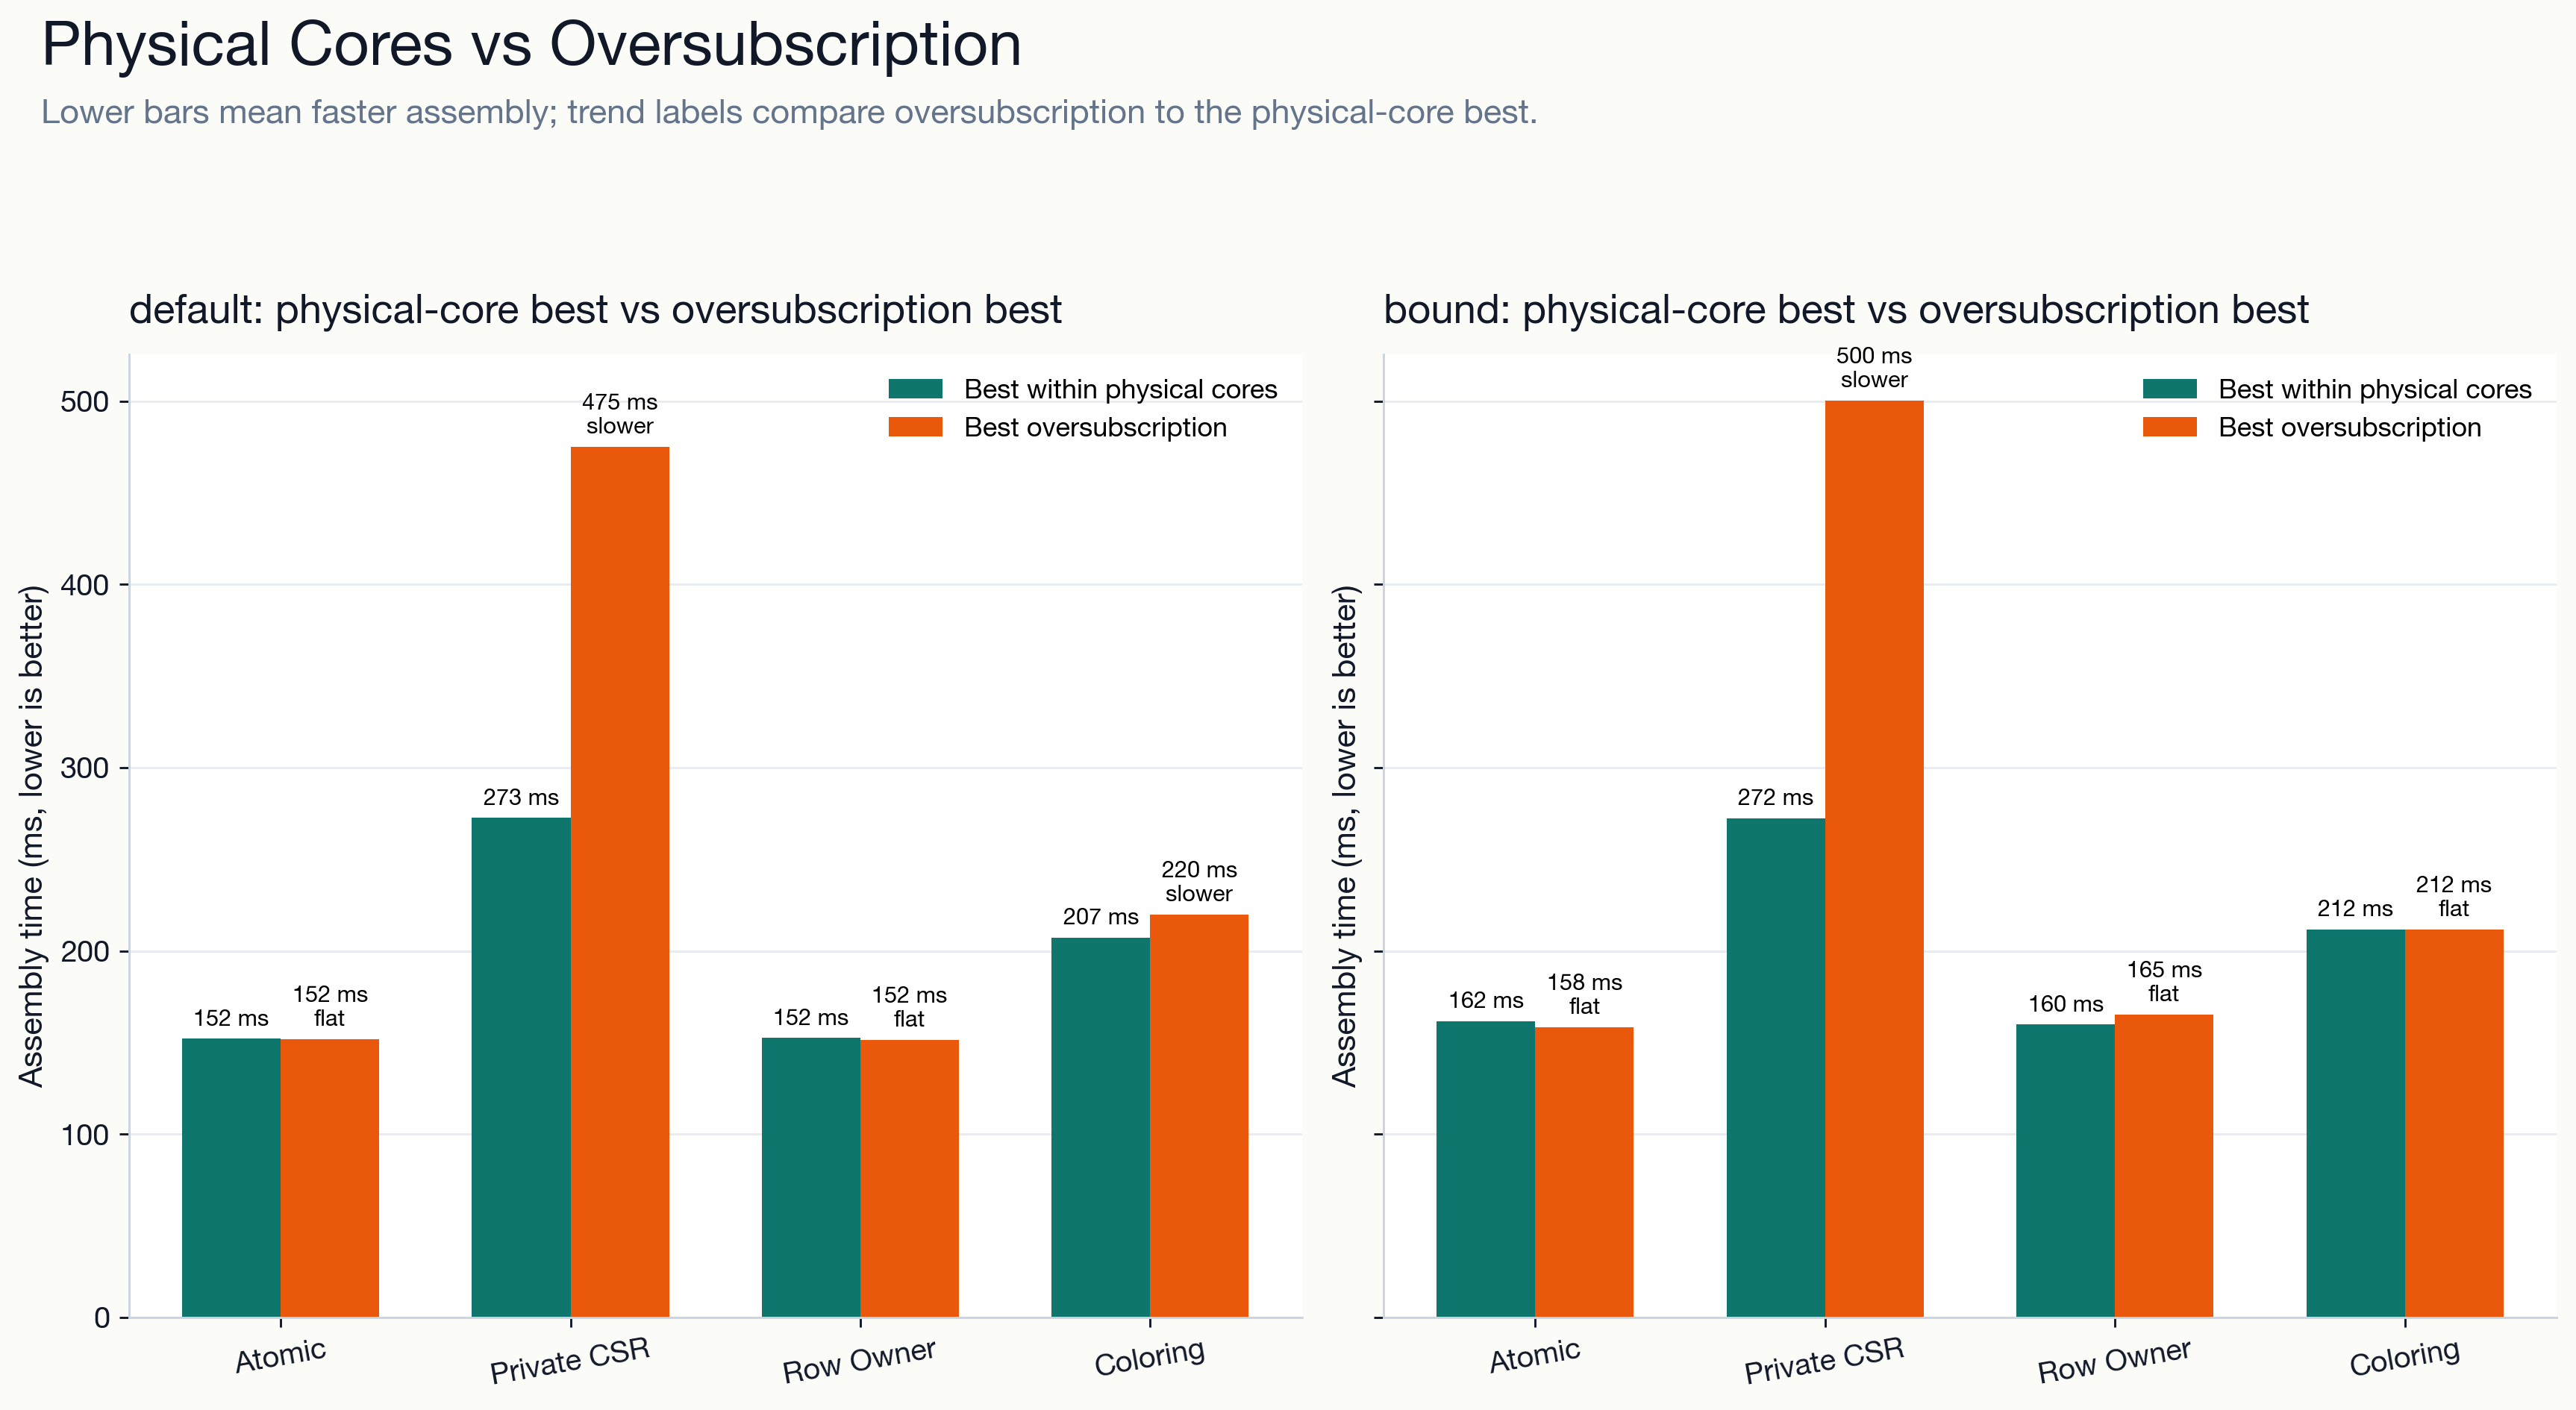
\includegraphics[width=\textwidth,height=0.62\textheight,keepaspectratio]{assets/intel_full_physical_vs_oversubscription.png}
\textbf{Intel full host}
\end{column}
\begin{column}{0.49\textwidth}
\centering
  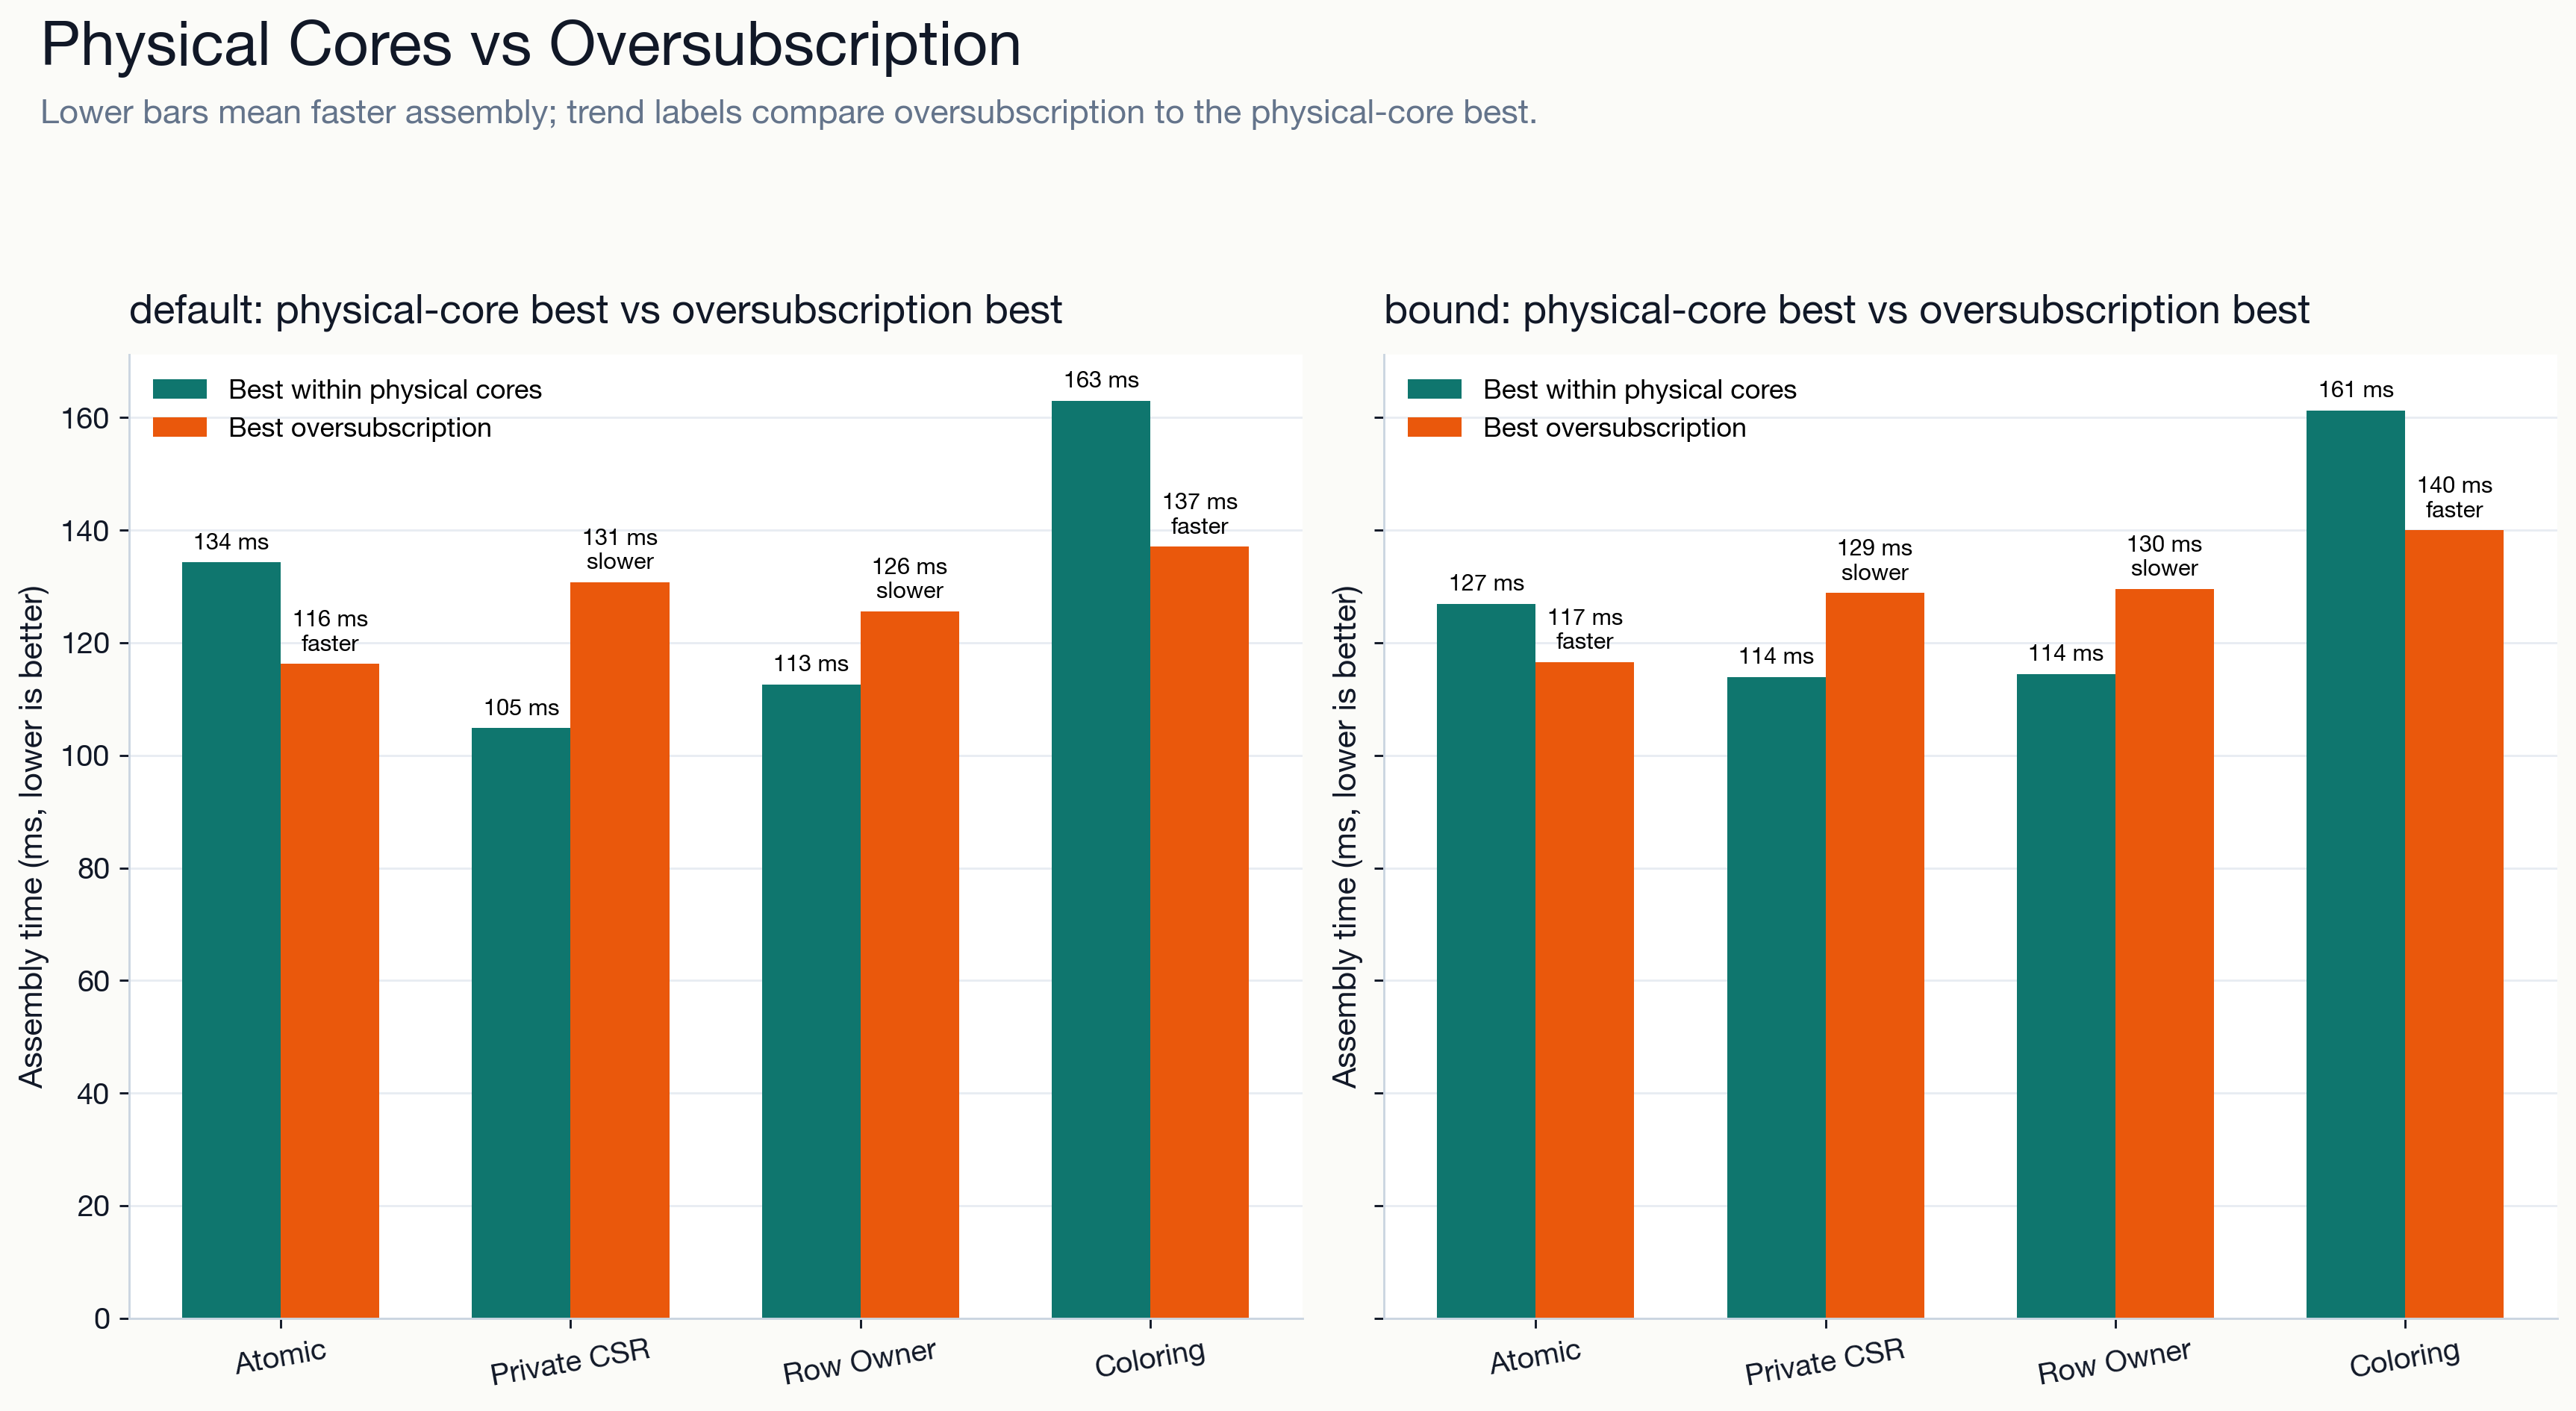
\includegraphics[width=\textwidth,height=0.62\textheight,keepaspectratio]{assets/apple_full_physical_vs_oversubscription.png}
\textbf{Apple M4 Max full host}
\end{column}
\end{columns}
\vspace{0.4em}
当前记录中 Intel 和 Apple 都是 \texttt{physical\_cores == logical\_cores}；超过物理核后的线程数只能解释为 \warn{软件线程过量订阅}。
\end{frame}
\note{
这一页回答 mentor 提到的物理核和逻辑核问题。这里的关键句是 \texttt{physical\_cores == logical\_cores}。也就是说，当前两个平台的实验记录里，没有暴露 SMT 或 hyper-threading 形式的额外逻辑核。因此，如果线程数超过物理核心数，它不是在使用“逻辑核加速”，而是软件线程数量超过了硬件执行资源，属于 oversubscription。图里的目的就是比较物理核内最佳点和过量订阅区间的表现。讲的时候要避免说“逻辑核有效或无效”，只能说“这组平台没有真实逻辑核区间，因此无法从这里得出 SMT 收益结论”。
}

\begin{frame}{跨平台图只用于说明边界，不做绝对排名}
\begin{columns}[T,onlytextwidth]
\begin{column}{0.49\textwidth}
\centering
  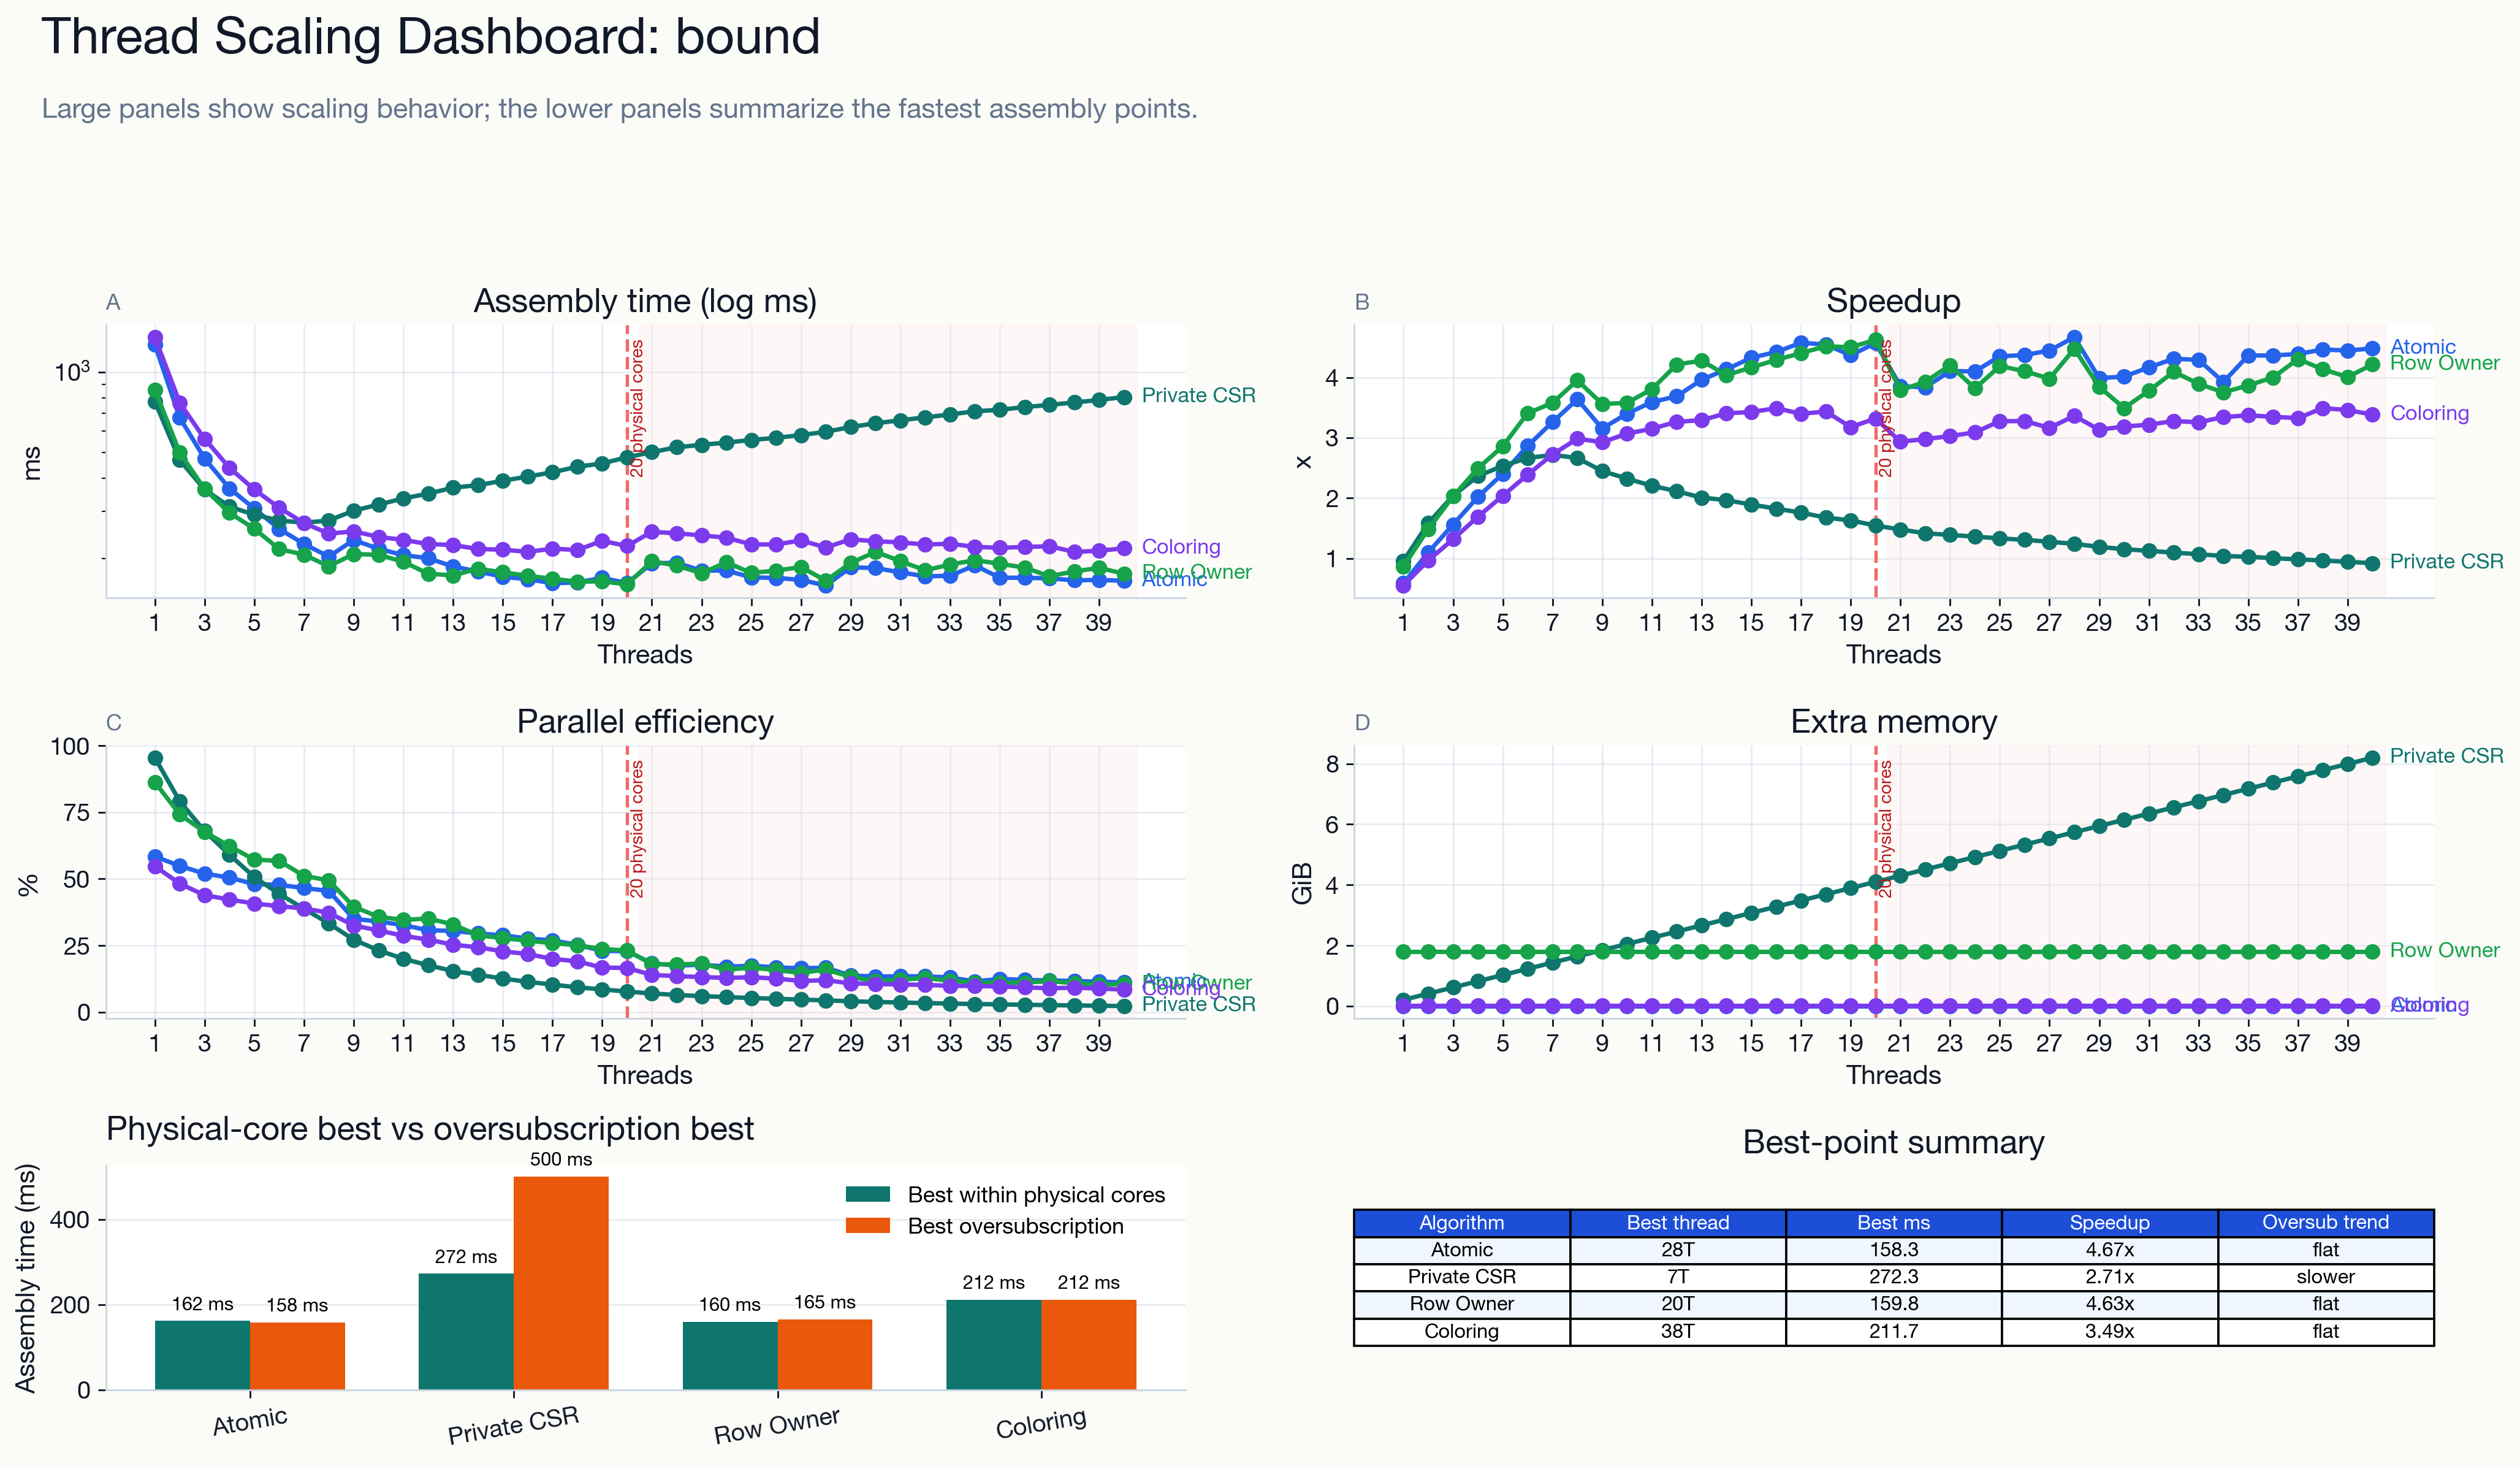
\includegraphics[width=\textwidth,height=0.62\textheight,keepaspectratio]{assets/intel_full_bound_dashboard.png}
\textbf{Intel full host}
\end{column}
\begin{column}{0.49\textwidth}
\centering
  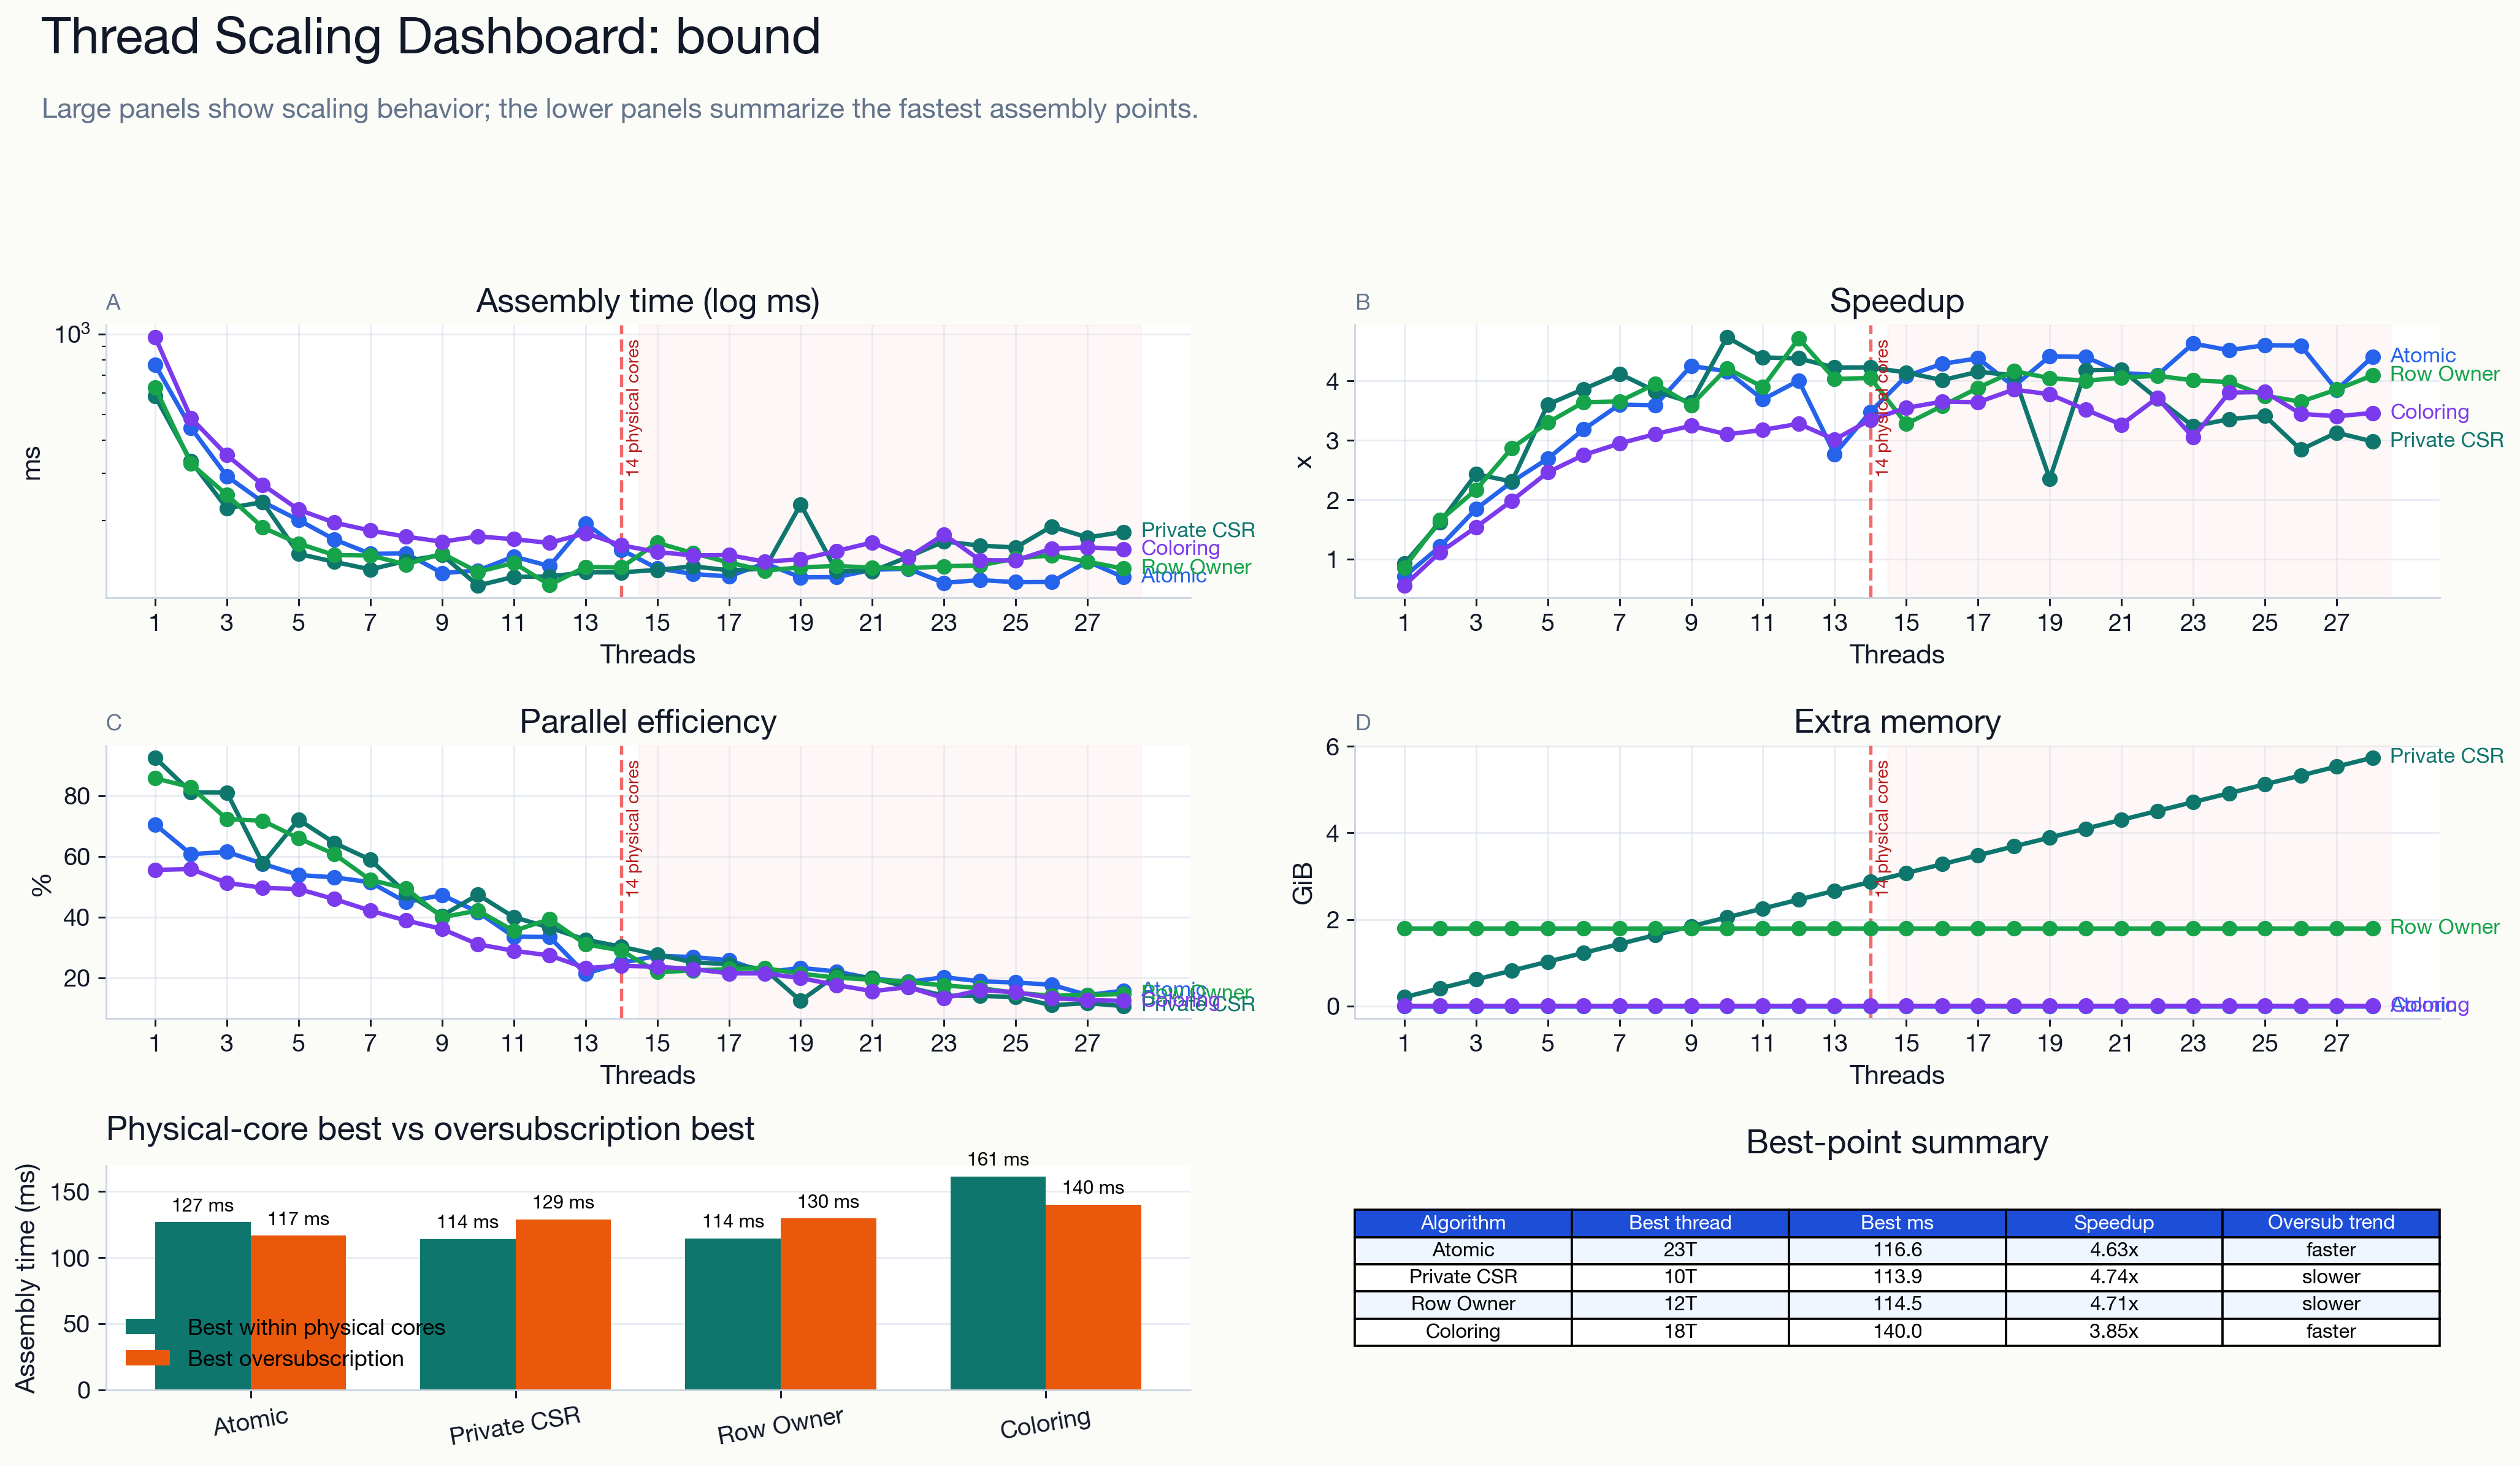
\includegraphics[width=\textwidth,height=0.62\textheight,keepaspectratio]{assets/apple_full_bound_dashboard.png}
\textbf{Apple M4 Max full host}
\end{column}
\end{columns}
\vspace{0.4em}
这两张图放在一起，是为了说明实验矩阵和趋势；硬件、OS、compiler、OpenMP runtime 和 affinity 控制都不同，不能直接写成纯算法排名。
\end{frame}
\note{
这页把 Intel 和 Apple 的 full-host bound dashboard 放在一起。bound 表示用了 \texttt{OMP\_PROC\_BIND=close} 和 \texttt{OMP\_PLACES=cores} 这类绑定设置。讲图时可以指出每个平台内部可以比较不同算法的趋势，但跨平台绝对时间不能直接说明某个算法在所有机器上更好。原因是 CPU 架构、操作系统调度、编译器、OpenMP runtime 和内存系统都不同。这里图的价值是让 mentor 看到我们已经把跨平台 schema 和 profile 记录打通了，下一步可以更规范地扩展更多平台。
}

\begin{frame}{现在可以给 mentor 的阶段性答复}
\begin{columns}[T,onlytextwidth]
\begin{column}{0.50\textwidth}
\textbf{已经有数据支撑的部分}
\begin{itemize}
  \item 单次和多次组装：符号复用收益明确。
  \item 有符号和无符号：排序归并是直接路径的主要成本。
  \item Intel 主平台：full-host、P-core-only、E-core-only 已有实测图。
  \item Apple 对照平台：QoS-biased 结果用于说明调度边界。
  \item 物理核/逻辑核：当前没有 SMT 逻辑核收益证据。
\end{itemize}
\end{column}
\begin{column}{0.46\textwidth}
\textbf{接下来值得继续做的部分}
\begin{itemize}
  \item 在 Intel 上补同口径符号/无符号效率复测。
  \item 并行化 CSR/scatter 符号构建。
  \item 明确符号 artifact 生命周期，研究符号和数值阶段能否流水并行。
  \item 补充有 SMT 的 CPU，单独回答逻辑核收益。
\end{itemize}
\end{column}
\end{columns}
\end{frame}
\note{
这一页适合在进入结论前停一下，把“现在能说什么”和“不能过度说什么”分开。左边都是已有数据可以支撑的结论：符号复用有收益，无符号直接路径主要慢在排序归并；Intel 主平台已经有 full-host、P-core-only、E-core-only 实测图；Apple 对照平台的 QoS-biased 结果用于说明调度边界；当前平台没有 SMT 逻辑核收益证据。右边是下一步：第一，为了完全闭环，应在 Intel 上补同口径符号/无符号效率复测，而不是把 Apple 计时当成 Intel 计时；第二，符号阶段本身现在仍有 CSR 和 scatter 构建成本，可以考虑并行化；第三，研究符号 artifact 的生命周期，看能否和数值组装解耦甚至流水；第四，找一台有 SMT 的 CPU，才能真正回答逻辑核收益。
}

\begin{frame}{结论：先复用结构，再谈并行扩展}
\begin{enumerate}
  \item \keyword{二阶段组装在当前 C++ 平台里有明确实现}：CSR sparsity + scatter plan 是符号阶段，\texttt{Ke} 计算与 value 填充是数值阶段。
  \item \keyword{符号复用同时改善单次和多次组装}：WindHub + \texttt{physics\_tet4} 下，相对无符号直接组装从 \metric{1.644x} 提升到 \metric{8.086x}。
  \item \keyword{无符号直接路径的主要成本是排序归并}：每次约 5 秒量级，并且需要更高 transient memory。
  \item \keyword{硬件适配优先看 Intel 主平台}：已有 full-host、P-core-only、E-core-only 实测结果；Apple QoS profile 只作为跨平台调度边界。
  \item \keyword{下一步补齐 Intel 同口径效率表}：不要用 Apple 的符号/无符号计时替代 Intel 绝对性能。
\end{enumerate}
\end{frame}
\note{
结论页建议按五句话讲。第一句：这个项目不是停留在概念上，符号阶段和数值阶段在 C++ 里已经有对应实现。第二句：最重要的数字是 1.644x 到 8.086x，说明单次有收益，多次更明显，但这组数字来自 Apple M4 Max。第三句：无符号直接组装慢的主要原因不是 Ke 计算，而是贡献生成后的排序归并和临时内存。第四句：硬件适配优先看 Intel 主平台，因为已有 full-host、P-core-only、E-core-only 实测结果，Apple QoS profile 只用来说明跨平台调度机制不同。第五句：如果要把效率结论完全落到 Intel 用户平台，下一步应在 Intel 上补同口径符号/无符号效率复测，而不是用 Apple 时间替代 Intel 时间。
}

\appendix

\begin{frame}{附录：Apple Performance QoS bound dashboard}
\centering
\fitfig{0.93}{assets/apple_performance_qos_bound_dashboard.png}
\smallsource{2026-05-14-thread-scaling-macos-m4max-performance-qos}
\end{frame}
\note{
这页是 Apple Performance QoS profile。它不是硬绑 P-core，而是正常前台或偏性能的调度条件，线程范围限制在性能核心数量附近。图的用途是看在更偏性能核心资源时，各算法 bound 环境下的最好点和内存情况。讲时要再次提醒：Apple profile 的解释要比 Intel 更保守。
}

\begin{frame}{附录：Apple Efficiency QoS bound dashboard}
\centering
\fitfig{0.93}{assets/apple_efficiency_qos_bound_dashboard.png}
\smallsource{2026-05-14-thread-scaling-macos-m4max-efficiency-qos}
\end{frame}
\note{
这页是 Apple Efficiency QoS profile，使用 background policy 做调度偏置，并把线程范围限制在能效核心数量附近。图里时间会明显变慢，这说明核心资源和调度策略对组装性能很敏感。但不要把它说成严格 E-core-only throughput，因为 macOS 没有提供和 taskset 一样的硬限制。它适合作为敏感性实验，而不是硬件排名。
}

\begin{frame}{复现方式和这份材料的边界}
\begin{itemize}
  \item 这份材料包含 beamer 源码、核心图片资产和资产清单。
  \item 推荐使用 XeLaTeX 编译：\texttt{latexmk -xelatex -interaction=nonstopmode -halt-on-error mentor\_next\_steps\_beamer.tex}
  \item 当前机器缺少 \texttt{latexmk} / \texttt{xelatex} / \texttt{pdflatex}，所以这里只做源码、路径和引用检查。
  \item 所有图片均来自仓库已有结果目录；没有新增 benchmark，也没有新生成数据图。
\end{itemize}
\end{frame}
\note{
最后一页用于交代交付边界。普通汇报时这页可以不讲，除非 mentor 问 PDF 或图表是怎么生成的。需要说明：这份材料是 beamer 源码包，中文需要 XeLaTeX；当前机器没有 TeX 编译工具，所以没有在本地生成 PDF。所有图都来自已有 result 目录，没有为了这份 slides 重新跑 benchmark，也没有新画数据图。这样可以保证材料里的数字和图表都可追溯。
}

\end{document}
